% Options for packages loaded elsewhere
\PassOptionsToPackage{unicode}{hyperref}
\PassOptionsToPackage{hyphens}{url}
%
\documentclass[
]{article}
\usepackage{amsmath,amssymb}
\usepackage{lmodern}
\usepackage{ifxetex,ifluatex}
\ifnum 0\ifxetex 1\fi\ifluatex 1\fi=0 % if pdftex
  \usepackage[T1]{fontenc}
  \usepackage[utf8]{inputenc}
  \usepackage{textcomp} % provide euro and other symbols
\else % if luatex or xetex
  \usepackage{unicode-math}
  \defaultfontfeatures{Scale=MatchLowercase}
  \defaultfontfeatures[\rmfamily]{Ligatures=TeX,Scale=1}
\fi
% Use upquote if available, for straight quotes in verbatim environments
\IfFileExists{upquote.sty}{\usepackage{upquote}}{}
\IfFileExists{microtype.sty}{% use microtype if available
  \usepackage[]{microtype}
  \UseMicrotypeSet[protrusion]{basicmath} % disable protrusion for tt fonts
}{}
\makeatletter
\@ifundefined{KOMAClassName}{% if non-KOMA class
  \IfFileExists{parskip.sty}{%
    \usepackage{parskip}
  }{% else
    \setlength{\parindent}{0pt}
    \setlength{\parskip}{6pt plus 2pt minus 1pt}}
}{% if KOMA class
  \KOMAoptions{parskip=half}}
\makeatother
\usepackage{xcolor}
\IfFileExists{xurl.sty}{\usepackage{xurl}}{} % add URL line breaks if available
\IfFileExists{bookmark.sty}{\usepackage{bookmark}}{\usepackage{hyperref}}
\hypersetup{
  pdftitle={Análise Descritiva das Variantes de COVID-19},
  pdfauthor={Elias Ribeiro},
  hidelinks,
  pdfcreator={LaTeX via pandoc}}
\urlstyle{same} % disable monospaced font for URLs
\usepackage[margin=1in]{geometry}
\usepackage{color}
\usepackage{fancyvrb}
\newcommand{\VerbBar}{|}
\newcommand{\VERB}{\Verb[commandchars=\\\{\}]}
\DefineVerbatimEnvironment{Highlighting}{Verbatim}{commandchars=\\\{\}}
% Add ',fontsize=\small' for more characters per line
\usepackage{framed}
\definecolor{shadecolor}{RGB}{248,248,248}
\newenvironment{Shaded}{\begin{snugshade}}{\end{snugshade}}
\newcommand{\AlertTok}[1]{\textcolor[rgb]{0.94,0.16,0.16}{#1}}
\newcommand{\AnnotationTok}[1]{\textcolor[rgb]{0.56,0.35,0.01}{\textbf{\textit{#1}}}}
\newcommand{\AttributeTok}[1]{\textcolor[rgb]{0.77,0.63,0.00}{#1}}
\newcommand{\BaseNTok}[1]{\textcolor[rgb]{0.00,0.00,0.81}{#1}}
\newcommand{\BuiltInTok}[1]{#1}
\newcommand{\CharTok}[1]{\textcolor[rgb]{0.31,0.60,0.02}{#1}}
\newcommand{\CommentTok}[1]{\textcolor[rgb]{0.56,0.35,0.01}{\textit{#1}}}
\newcommand{\CommentVarTok}[1]{\textcolor[rgb]{0.56,0.35,0.01}{\textbf{\textit{#1}}}}
\newcommand{\ConstantTok}[1]{\textcolor[rgb]{0.00,0.00,0.00}{#1}}
\newcommand{\ControlFlowTok}[1]{\textcolor[rgb]{0.13,0.29,0.53}{\textbf{#1}}}
\newcommand{\DataTypeTok}[1]{\textcolor[rgb]{0.13,0.29,0.53}{#1}}
\newcommand{\DecValTok}[1]{\textcolor[rgb]{0.00,0.00,0.81}{#1}}
\newcommand{\DocumentationTok}[1]{\textcolor[rgb]{0.56,0.35,0.01}{\textbf{\textit{#1}}}}
\newcommand{\ErrorTok}[1]{\textcolor[rgb]{0.64,0.00,0.00}{\textbf{#1}}}
\newcommand{\ExtensionTok}[1]{#1}
\newcommand{\FloatTok}[1]{\textcolor[rgb]{0.00,0.00,0.81}{#1}}
\newcommand{\FunctionTok}[1]{\textcolor[rgb]{0.00,0.00,0.00}{#1}}
\newcommand{\ImportTok}[1]{#1}
\newcommand{\InformationTok}[1]{\textcolor[rgb]{0.56,0.35,0.01}{\textbf{\textit{#1}}}}
\newcommand{\KeywordTok}[1]{\textcolor[rgb]{0.13,0.29,0.53}{\textbf{#1}}}
\newcommand{\NormalTok}[1]{#1}
\newcommand{\OperatorTok}[1]{\textcolor[rgb]{0.81,0.36,0.00}{\textbf{#1}}}
\newcommand{\OtherTok}[1]{\textcolor[rgb]{0.56,0.35,0.01}{#1}}
\newcommand{\PreprocessorTok}[1]{\textcolor[rgb]{0.56,0.35,0.01}{\textit{#1}}}
\newcommand{\RegionMarkerTok}[1]{#1}
\newcommand{\SpecialCharTok}[1]{\textcolor[rgb]{0.00,0.00,0.00}{#1}}
\newcommand{\SpecialStringTok}[1]{\textcolor[rgb]{0.31,0.60,0.02}{#1}}
\newcommand{\StringTok}[1]{\textcolor[rgb]{0.31,0.60,0.02}{#1}}
\newcommand{\VariableTok}[1]{\textcolor[rgb]{0.00,0.00,0.00}{#1}}
\newcommand{\VerbatimStringTok}[1]{\textcolor[rgb]{0.31,0.60,0.02}{#1}}
\newcommand{\WarningTok}[1]{\textcolor[rgb]{0.56,0.35,0.01}{\textbf{\textit{#1}}}}
\usepackage{graphicx}
\makeatletter
\def\maxwidth{\ifdim\Gin@nat@width>\linewidth\linewidth\else\Gin@nat@width\fi}
\def\maxheight{\ifdim\Gin@nat@height>\textheight\textheight\else\Gin@nat@height\fi}
\makeatother
% Scale images if necessary, so that they will not overflow the page
% margins by default, and it is still possible to overwrite the defaults
% using explicit options in \includegraphics[width, height, ...]{}
\setkeys{Gin}{width=\maxwidth,height=\maxheight,keepaspectratio}
% Set default figure placement to htbp
\makeatletter
\def\fps@figure{htbp}
\makeatother
\setlength{\emergencystretch}{3em} % prevent overfull lines
\providecommand{\tightlist}{%
  \setlength{\itemsep}{0pt}\setlength{\parskip}{0pt}}
\setcounter{secnumdepth}{-\maxdimen} % remove section numbering
\usepackage{booktabs}
\usepackage{longtable}
\usepackage{array}
\usepackage{multirow}
\usepackage{wrapfig}
\usepackage{float}
\usepackage{colortbl}
\usepackage{pdflscape}
\usepackage{tabu}
\usepackage{threeparttable}
\usepackage{threeparttablex}
\usepackage[normalem]{ulem}
\usepackage{makecell}
\usepackage{xcolor}
\ifluatex
  \usepackage{selnolig}  % disable illegal ligatures
\fi

\title{Análise Descritiva das Variantes de COVID-19}
\author{Elias Ribeiro}
\date{15/02/2022}

\begin{document}
\maketitle

{
\setcounter{tocdepth}{1}
\tableofcontents
}
\newpage

\hypertarget{os-dados.}{%
\section{Os dados.}\label{os-dados.}}

Neste Relatório iremos fazer uma análise descritiva das variantes de
COVID-19 dividas pelos períodos correspondentes a fim de tentar
identificar padrões das variantes em relação ao numero de casos, obitos
e internações. Estabelecemos a data pra variante delta de acordo com o
site:
\url{https://agenciabrasil.ebc.com.br/saude/noticia/2021-11/pesquisa-mapeia-entrada-e-disseminacao-da-variante-delta-no-brasil\#}
onde ele cita que a variante delta predominou no estado de São Paulo
desde a 33ª semana epidemiológica (15 a 21/8).

\begin{Shaded}
\begin{Highlighting}[]
\CommentTok{\#dados filtrados e tratados observatório 09/02/2022}
\NormalTok{dados }\OtherTok{\textless{}{-}} \FunctionTok{read\_excel}\NormalTok{(}\StringTok{"dados5.xlsx"}\NormalTok{)}

\CommentTok{\#criando variável chamada variante(original,gama,delta,omicron)}
\NormalTok{in\_gama }\OtherTok{\textless{}{-}} \FunctionTok{as.Date}\NormalTok{(}\StringTok{"01{-}01{-}2021"}\NormalTok{,}\AttributeTok{format=}\StringTok{"\%d{-}\%m{-}\%Y"}\NormalTok{)}
\NormalTok{in\_delta }\OtherTok{\textless{}{-}} \FunctionTok{as.Date}\NormalTok{(}\StringTok{"15{-}08{-}2021"}\NormalTok{,}\AttributeTok{format=}\StringTok{"\%d{-}\%m{-}\%Y"}\NormalTok{)}
\NormalTok{in\_ommi }\OtherTok{\textless{}{-}} \FunctionTok{as.Date}\NormalTok{(}\StringTok{"01{-}01{-}2022"}\NormalTok{,}\AttributeTok{format=}\StringTok{"\%d{-}\%m{-}\%Y"}\NormalTok{)}
\NormalTok{dados }\OtherTok{\textless{}{-}}\NormalTok{ dados }\SpecialCharTok{\%\textgreater{}\%} 
  \FunctionTok{mutate}\NormalTok{(}\AttributeTok{variante =} \FunctionTok{case\_when}\NormalTok{(dt\_sint }\SpecialCharTok{\textless{}}\NormalTok{ in\_gama }\SpecialCharTok{\textasciitilde{}} \StringTok{"original"}\NormalTok{,}
\NormalTok{                              dt\_sint }\SpecialCharTok{\textgreater{}=}\NormalTok{ in\_gama }\SpecialCharTok{\&}\NormalTok{ dt\_sint }\SpecialCharTok{\textless{}}\NormalTok{ in\_delta }\SpecialCharTok{\textasciitilde{}} \StringTok{"gama"}\NormalTok{,}
\NormalTok{                              dt\_sint }\SpecialCharTok{\textgreater{}=}\NormalTok{ in\_delta }\SpecialCharTok{\&}\NormalTok{ dt\_sint }\SpecialCharTok{\textless{}}\NormalTok{ in\_ommi }\SpecialCharTok{\textasciitilde{}} \StringTok{"delta"}\NormalTok{,}
\NormalTok{                              dt\_sint }\SpecialCharTok{\textgreater{}=}\NormalTok{ in\_ommi }\SpecialCharTok{\textasciitilde{}} \StringTok{"omicron"}\NormalTok{)) }\SpecialCharTok{\%\textgreater{}\%} 
  \FunctionTok{mutate}\NormalTok{(}\AttributeTok{month\_year =} \FunctionTok{paste}\NormalTok{(}\FunctionTok{formatC}\NormalTok{(}\FunctionTok{month}\NormalTok{(dt\_sint), }\AttributeTok{width=}\DecValTok{2}\NormalTok{, }\AttributeTok{format=}\StringTok{"d"}\NormalTok{, }\AttributeTok{flag=}\StringTok{"0"}\NormalTok{),}
                            \FunctionTok{year}\NormalTok{(dt\_sint),}\AttributeTok{sep=}\StringTok{"/"}\NormalTok{)) }\SpecialCharTok{\%\textgreater{}\%} 
  \FunctionTok{mutate}\NormalTok{(}\AttributeTok{mes =} \FunctionTok{month}\NormalTok{(dt\_sint))}
\end{Highlighting}
\end{Shaded}

\hypertarget{frequuxeancia-variantes}{%
\section{Frequência Variantes}\label{frequuxeancia-variantes}}

\begin{Shaded}
\begin{Highlighting}[]
\NormalTok{dados }\OtherTok{\textless{}{-}}
\NormalTok{  dados }\SpecialCharTok{\%\textgreater{}\%} \FunctionTok{mutate}\NormalTok{(}
    \AttributeTok{classi\_fin =} \FunctionTok{case\_when}\NormalTok{(}
\NormalTok{      CLASSI\_FIN }\SpecialCharTok{==} \DecValTok{5} \SpecialCharTok{\textasciitilde{}} \StringTok{"COVID{-}19"}\NormalTok{,}
\NormalTok{      CLASSI\_FIN }\SpecialCharTok{==} \DecValTok{1} \SpecialCharTok{\textasciitilde{}} \StringTok{"Influenza"}\NormalTok{,}
\NormalTok{      CLASSI\_FIN }\SpecialCharTok{==} \DecValTok{2} \SpecialCharTok{\textasciitilde{}} \StringTok{"Outro vírus"}\NormalTok{,}
\NormalTok{      CLASSI\_FIN }\SpecialCharTok{==} \DecValTok{3} \SpecialCharTok{\textasciitilde{}} \StringTok{"Outro agente"}\NormalTok{,}
\NormalTok{      CLASSI\_FIN }\SpecialCharTok{==} \DecValTok{4} \SpecialCharTok{\textasciitilde{}} \StringTok{"Não especificado"}\NormalTok{,}
      \ConstantTok{TRUE} \SpecialCharTok{\textasciitilde{}} \ConstantTok{NA\_character\_}
\NormalTok{    )}
\NormalTok{  )}

\FunctionTok{with}\NormalTok{(dados, }\FunctionTok{ctable}\NormalTok{(classi\_fin, variante, }\AttributeTok{prop =} \StringTok{"c"}\NormalTok{, }\AttributeTok{useNA =} \StringTok{"no"}\NormalTok{)) }\SpecialCharTok{\%\textgreater{}\%} \FunctionTok{kable}\NormalTok{()}
\end{Highlighting}
\end{Shaded}

\begin{table}

\centering
\begin{tabular}[t]{l|r|r|r|r|r}
\hline
  & delta & gama & omicron & original & Total\\
\hline
COVID-19 & 1228 & 11160 & 1353 & 6852 & 20593\\
\hline
Influenza & 363 & 9 & 116 & 84 & 572\\
\hline
Não especificado & 1997 & 4272 & 415 & 6774 & 13458\\
\hline
Outro agente & 19 & 24 & 0 & 40 & 83\\
\hline
Outro vírus & 73 & 149 & 2 & 84 & 308\\
\hline
Total & 3680 & 15614 & 1886 & 13834 & 35014\\
\hline
\end{tabular}
\centering
\begin{tabular}[t]{l|r|r|r|r|r}
\hline
  & delta & gama & omicron & original & Total\\
\hline
COVID-19 & 0.3336957 & 0.7147432 & 0.7173913 & 0.4953014 & 0.5881362\\
\hline
Influenza & 0.0986413 & 0.0005764 & 0.0615058 & 0.0060720 & 0.0163363\\
\hline
Não especificado & 0.5426630 & 0.2736006 & 0.2200424 & 0.4896631 & 0.3843605\\
\hline
Outro agente & 0.0051630 & 0.0015371 & 0.0000000 & 0.0028914 & 0.0023705\\
\hline
Outro vírus & 0.0198370 & 0.0095427 & 0.0010604 & 0.0060720 & 0.0087965\\
\hline
Total & 1.0000000 & 1.0000000 & 1.0000000 & 1.0000000 & 1.0000000\\
\hline
\end{tabular}
\end{table}

\begin{Shaded}
\begin{Highlighting}[]
\NormalTok{dados }\OtherTok{\textless{}{-}}\NormalTok{ dados }\SpecialCharTok{\%\textgreater{}\%} 
  \FunctionTok{filter}\NormalTok{(CLASSI\_FIN }\SpecialCharTok{==} \StringTok{"5"}\NormalTok{)}

\FunctionTok{freq}\NormalTok{(dados}\SpecialCharTok{$}\NormalTok{variante) }
\end{Highlighting}
\end{Shaded}

\begin{verbatim}
## Frequencies  
## dados$variante  
## Type: Character  
## 
##                   Freq   % Valid   % Valid Cum.   % Total   % Total Cum.
## -------------- ------- --------- -------------- --------- --------------
##          delta    1228      5.96           5.96      5.96           5.96
##           gama   11160     54.19          60.16     54.19          60.16
##        omicron    1353      6.57          66.73      6.57          66.73
##       original    6852     33.27         100.00     33.27         100.00
##           <NA>       0                               0.00         100.00
##          Total   20593    100.00         100.00    100.00         100.00
\end{verbatim}

Agora vamos fazer os gŕaficos de casos, obitos e internações para tentar
identificarmos as variantes ao longo do tempo.

\hypertarget{casos-covid-19-por-muxeas}{%
\section{Casos COVID-19 por mês}\label{casos-covid-19-por-muxeas}}

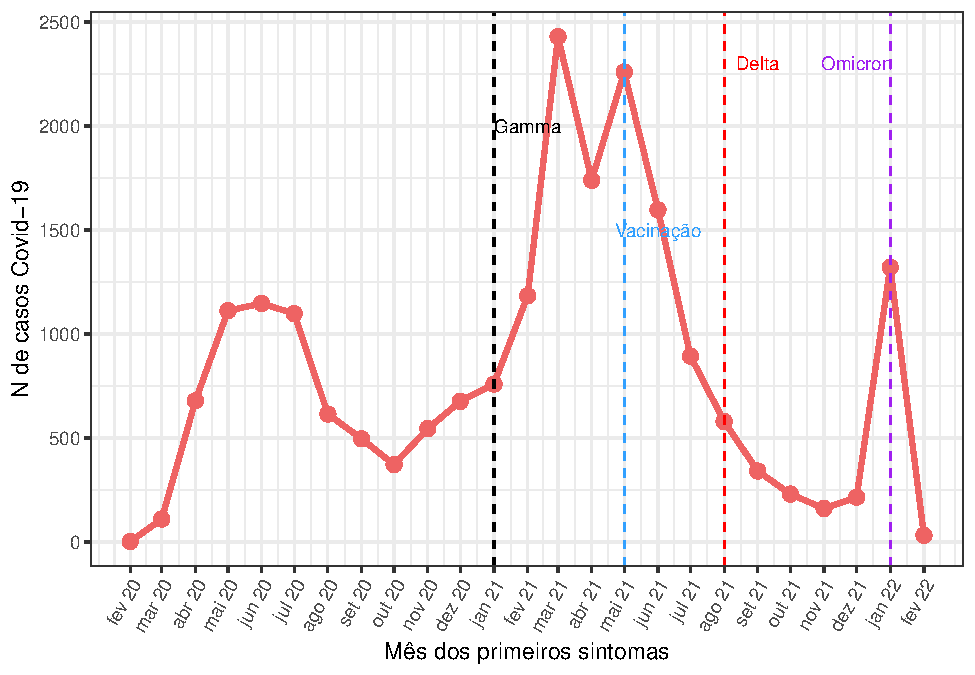
\includegraphics{analises_variantes_files/figure-latex/unnamed-chunk-3-1.pdf}

\begin{verbatim}
##    Mês  Ano Numero de casos
## 1   02 2020               2
## 2   03 2020             110
## 3   04 2020             679
## 4   05 2020            1112
## 5   06 2020            1147
## 6   07 2020            1098
## 7   08 2020             615
## 8   09 2020             496
## 9   10 2020             372
## 10  11 2020             545
## 11  12 2020             676
## 12  01 2021             759
## 13  02 2021            1184
## 14  03 2021            2430
## 15  04 2021            1739
## 16  05 2021            2260
## 17  06 2021            1597
## 18  07 2021             893
## 19  08 2021             579
## 20  09 2021             341
## 21  10 2021             230
## 22  11 2021             161
## 23  12 2021             215
## 24  01 2022            1321
## 25  02 2022              32
\end{verbatim}

\hypertarget{casos-de-uxf3bitos-covid-19-por-muxeas}{%
\section{Casos de óbitos COVID-19 por
mês}\label{casos-de-uxf3bitos-covid-19-por-muxeas}}

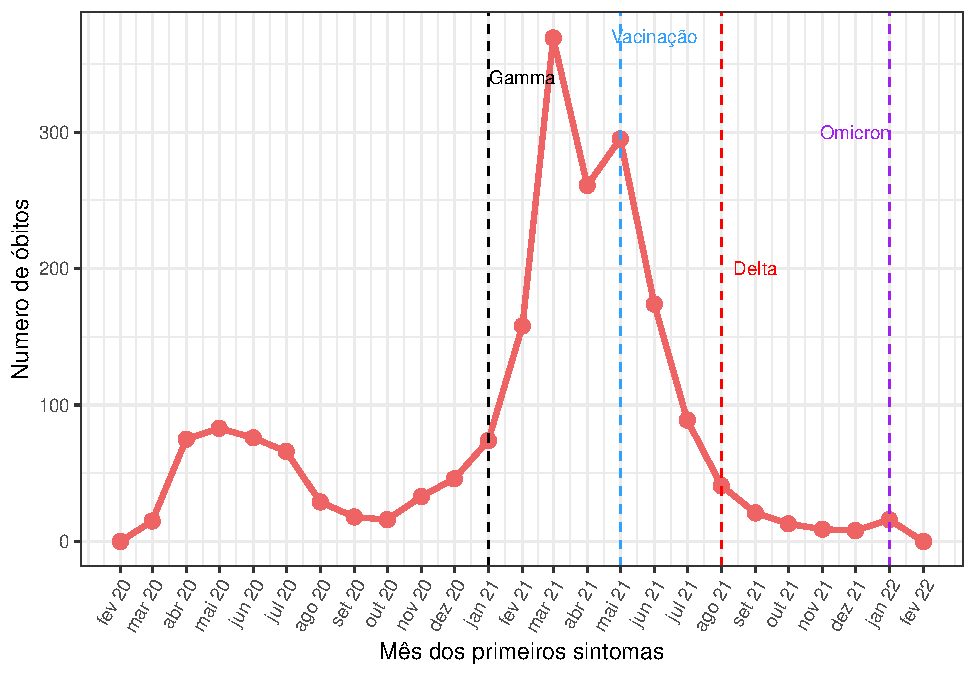
\includegraphics{analises_variantes_files/figure-latex/unnamed-chunk-4-1.pdf}

\hypertarget{letalidade-covid-19}{%
\section{Letalidade COVID-19}\label{letalidade-covid-19}}

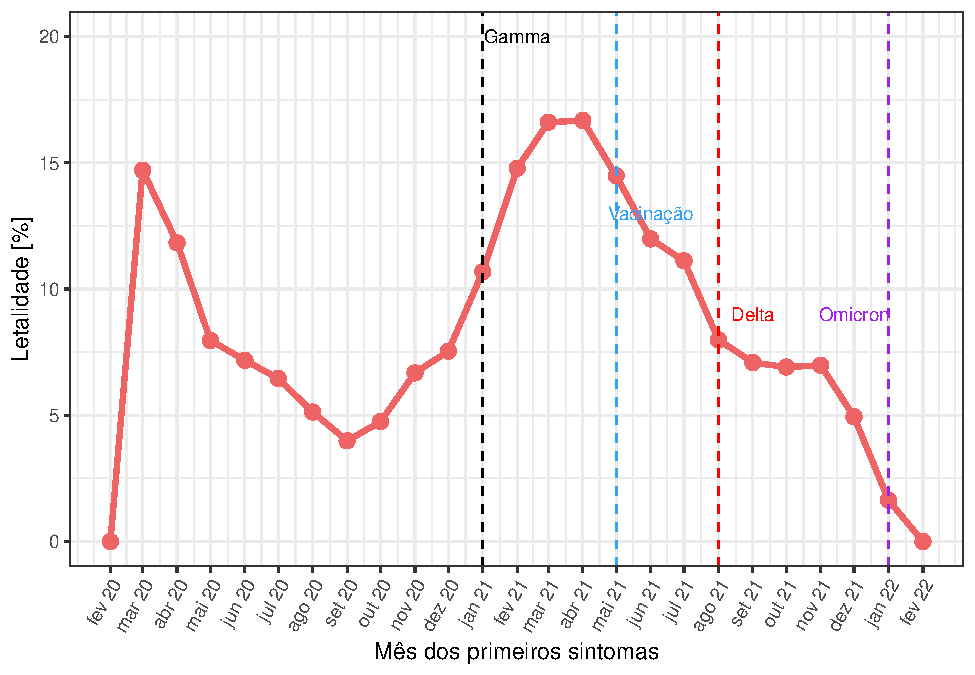
\includegraphics{analises_variantes_files/figure-latex/unnamed-chunk-5-1.pdf}

\begin{verbatim}
##    Mês  Ano obitos numero casos finalizados     %
## 1   02 2020      0                        1  0.00
## 2   03 2020     15                      102 14.71
## 3   04 2020     75                      634 11.83
## 4   05 2020     83                     1042  7.97
## 5   06 2020     76                     1059  7.18
## 6   07 2020     66                     1022  6.46
## 7   08 2020     29                      565  5.13
## 8   09 2020     18                      451  3.99
## 9   10 2020     16                      337  4.75
## 10  11 2020     33                      494  6.68
## 11  12 2020     46                      610  7.54
## 12  01 2021     74                      692 10.69
## 13  02 2021    158                     1068 14.79
## 14  03 2021    369                     2221 16.61
## 15  04 2021    261                     1565 16.68
## 16  05 2021    295                     2036 14.49
## 17  06 2021    174                     1451 11.99
## 18  07 2021     89                      800 11.12
## 19  08 2021     41                      513  7.99
## 20  09 2021     21                      296  7.09
## 21  10 2021     13                      188  6.91
## 22  11 2021      9                      129  6.98
## 23  12 2021      8                      162  4.94
## 24  01 2022     16                      973  1.64
## 25  02 2022      0                       11  0.00
\end{verbatim}

\hypertarget{casos-de-internauxe7uxf5es-na-uti-covid-19-por-muxeas}{%
\section{Casos de Internações na UTI COVID-19 por
mês}\label{casos-de-internauxe7uxf5es-na-uti-covid-19-por-muxeas}}

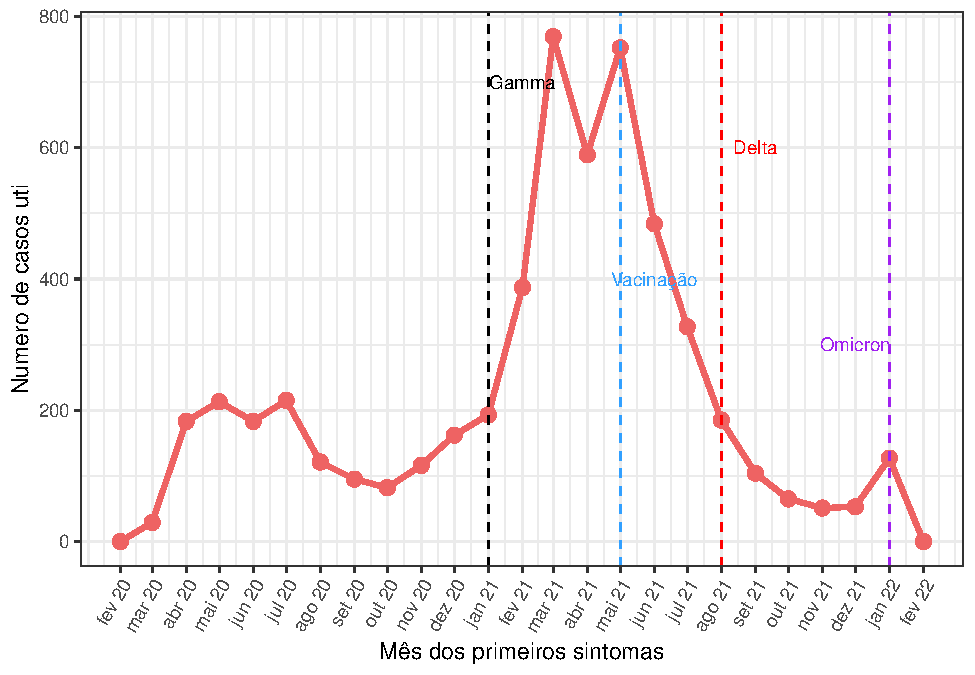
\includegraphics{analises_variantes_files/figure-latex/unnamed-chunk-6-1.pdf}

\begin{verbatim}
##    Mês  Ano n uti casos finalizados
## 1   02 2020     0                 2
## 2   03 2020    29                92
## 3   04 2020   183               599
## 4   05 2020   213               972
## 5   06 2020   183               999
## 6   07 2020   215               980
## 7   08 2020   121               549
## 8   09 2020    95               428
## 9   10 2020    82               337
## 10  11 2020   116               481
## 11  12 2020   162               600
## 12  01 2021   193               672
## 13  02 2021   387              1095
## 14  03 2021   769              2206
## 15  04 2021   589              1565
## 16  05 2021   752              2086
## 17  06 2021   484              1445
## 18  07 2021   327               807
## 19  08 2021   185               521
## 20  09 2021   104               313
## 21  10 2021    65               215
## 22  11 2021    51               144
## 23  12 2021    53               184
## 24  01 2022   127              1096
## 25  02 2022     0                25
\end{verbatim}

\end{document}
